\documentclass[a4paper,12pt]{article}

% Pour le bon support de la langue française : 
\usepackage[utf8]{inputenc}
\usepackage[T1]{fontenc}
\usepackage[francais]{babel}

\usepackage{lipsum} % \lipsum créera un texte test
\usepackage[margin=2.4cm]{geometry} %pour des marges

\usepackage{framed} % des contours
\usepackage[framed]{ntheorem} % un théoreme

\usepackage{algorithm}
\usepackage{algorithmic}

\makeatletter
\renewcommand{\ALG@name}{Algorithme}
\makeatother

\usepackage[all]{xy}
%
\usepackage{listings}

\usepackage{hyperref}
\hypersetup{
    bookmarks=true,         % show bookmarks bar?
    unicode=false,          % non-Latin characters in Acrobat’s bookmarks
    pdftoolbar=true,        % show Acrobat’s toolbar?
    pdfmenubar=true,        % show Acrobat’s menu?
    pdffitwindow=false,     % window fit to page when opened
    pdfstartview={FitH},    % fits the width of the page to the window
    pdfnewwindow=true,      % links in new PDF window
    colorlinks=true,       % false: boxed links; true: colored links
    linkcolor=blue,          % color of internal links (change box color with linkbordercolor)
    citecolor=green,        % color of links to bibliography
    filecolor=magenta,      % color of file links
    urlcolor=cyan           % color of external links
}

%\let\urlorig\url
%\renewcommand{\url}[1]{%
%   \begin{otherlanguage}{english}\urlorig{#1}\end{otherlanguage}%
%}


% Bibliographie dans la Table des matières
\usepackage[nottoc, notlof, notlot]{tocbibind}



\usepackage{tikz}               % Tracer des graphes
\tikzset{every picture/.style={execute at begin picture={
\shorthandoff{:;!?};}
}}


\usepackage{thumbpdf}           % Fichier pdf généré 
                                % contien une              
                                % miniature de chaque slide 

 \usepackage{dsfont}
\usepackage{lastpage}           % Avoir total de pages dans le footer.
\usepackage{graphicx}           % Pour les images et figures
\usepackage{wrapfig}            % Pour détourer les figures
\usepackage{fancybox}           % De chouettes encadrements
\usepackage{lettrine}           % Pour de beaux paragraphes
\usepackage{setspace}           % Pour changer l'interligne
\usepackage{eurosym}            % Pour le signe \euro
\usepackage{xcolor}             % Pour mettre d la couleur
\usepackage{colortbl}           % Couleur dans tableaux
\usepackage{tabularx}           % pour des tableaux à taille de la page
\usepackage{longtable}          % Pour les grands tableaux
\usepackage[tight]{shorttoc}    % Pour faire un sommaire à la française.
\newcommand{\sommaire}{\shorttoc{Sommaire}{1}}
\usepackage{array}              % De beaux tableaux
\usepackage{multirow}           % Tableaux sur plusieurs lignes
                                % \multirow{nlignes}{largeur ou *}{contenu}
\usepackage{amsmath}            % Un peu de maths
\usepackage{amssymb}            % Encore des maths
\usepackage{mathtools}
\usepackage{empheq}             % Pour encadrer les équations


\usepackage{stmaryrd}			% pour les crochets d'intervalles entiers 


\usepackage{pgfpages}           % Pour avoir 2 pages sur A4 paysage
\usepackage{datetime}           % Jouer facilement avec les dates
% Pour la physique : 
\usepackage{numprint}           % Pour faire des groupes de 3 nombres
\usepackage[squaren,Gray,cdot]{SIunits}

\usepackage{pgf}
\usetikzlibrary{arrows}

\usepackage{nameref} %pour les entetes 
\makeatletter
\newcommand*{\currentname}{\@currentlabelname}
\makeatother

\definecolor{vert}{rgb}{0,0.6,0}
\definecolor{mauve}{rgb}{0.58,0,0.82}

\lstset{ %
  backgroundcolor=\color{white},   % choose the background color
  breaklines=true,                 % automatic line breaking only at whitespace
  captionpos=b,                    % sets the caption-position to bottom
  commentstyle=\color{vert},    % comment style
  escapeinside={\%*}{*)},          % if you want to add LaTeX within your code
  keywordstyle=\color{blue},       % keyword style
  stringstyle=\color{mauve},     % string literal style
  basicstyle=\small\ttfamily,%
  frame=single,
  %extendedchars=true,
 literate=%
         {é}{{\'e}}1
         {É}{{\'E}}1
         {à}{{\`a}}1
         {ê}{{\^e}}1
         {è}{{\`e}}1
}

%%%
% Commandes
\newcommand{\ndiv}{\nmid} %x\ndiv y <==> x ne divise pas y
\newcommand{\modulo}[3]{#1\equiv #2 \;[#3]}
\newcommand{\nmodulo}[3]{#1\not\equiv #2 \;[#3]}


% Ajout d'une image avec label
\newcommand{\image}[3]{
% \image{fichier}{label}{description}
\begin{center}
% Nécessite le package float
\begin{figure}[H]
\includegraphics[width=0.9\textwidth]{#1}
\caption{\label{#2}{#3}}
\end{figure}
\end{center}
}

% Ajout d'une image largeur page avec label
\newcommand{\imagebig}[3]{
% \imagebig{fichier}{label}{description}
\begin{center}
% Nécessite le package float
\begin{figure}[H]
\includegraphics[width=\textwidth]{#1}
\caption{\label{#2}{#3}}
\end{figure}
\end{center}
}

% Une image qui prend toute la page
\newcommand{\imagefull}[1]{
    \newgeometry{margin=0cm}
\begin{center}
\begin{figure}[H]
\includegraphics[width=0.96\paperwidth]{#1}
\end{figure}
\end{center}
\restoregeometry
\nopagebreak
}

% Un encadré grisé
\newcommand{\encadregris}[1]{
\begin{center}
\colorbox{gray!20}{
\begin{minipage}{0.95\textwidth}
{#1}
\end{minipage}
}
\end{center}
}

% Un mot grisé
\newcommand{\motgris}[1]{
\colorbox{gray!20}{{#1}}
}

% Un encadré
\newcommand{\encadre}[1]{
\begin{center}
\fbox{
\begin{minipage}{\textwidth}
{#1}
\end{minipage}
}
\end{center}
}

%Une boite coloré
\newenvironment{colbox}[1]
{\def\FrameCommand{\colorbox{#1}}%
   \MakeFramed{\advance\hsize-\width \FrameRestore}}
{\endMakeFramed}

\colorlet{shadecolor}{blue!8}

%%%%%%%%%% Des Maths %%%%%%%%%%%%%%

\newcommand{\RR}{\ensuremath{\mathbb{R}}}
\newcommand{\CC}{\ensuremath{\mathbb{C}}}
\newcommand{\ZZ}{\ensuremath{\mathbb{Z}}}
\newcommand{\QQ}{\ensuremath{\mathbb{Q}}}
\newcommand{\NN}{\ensuremath{\mathbb{N}}}
\newcommand{\PP}{\ensuremath{\mathbb{P}}}
\newcommand{\KK}{\ensuremath{\mathbb{K}}}
\newcommand{\EE}{\ensuremath{\mathbb{E}}}
\renewcommand{\SS}{\ensuremath{\mathbb{S}}}
\newcommand{\TT}{\ensuremath{\mathbb{T}}}

\newcounter{theo}[section] % créer un nouveau compteur
\renewcommand\thetheo{\thesection.\arabic{theo}}
\newcounter{prop}[section]
\renewcommand\theprop{\thesection.\arabic{prop}}

\newenvironment{theoreme}[1]
{\refstepcounter{theo}\begin{shaded}\textbf{Théorème \thetheo~ : } \textit{#1}\vspace{0.3em}
\hrule
\medbreak}
{\end{shaded}}


\newenvironment{propriete}
{\begin{shaded}\textbf{Propriété : }\\ }
{\end{shaded}}

\newenvironment{proposition}
{\refstepcounter{prop}\begin{shaded}\textbf{Proposition \theprop~ : }\\ }
{\end{shaded}}

\newenvironment{corollaire}
{\begin{shaded}\textbf{Corollaire : }\\ }
{\end{shaded}}


\newenvironment{lemme}
{\begin{shaded}\textbf{Lemme : }\\ }
{\end{shaded}}


\newenvironment{definition}[1]
{\stepcounter{theo}\begin{shaded}\textbf{Définition \thetheo~ : } \textit{#1}\vspace{0.3em}
\hrule
\medbreak}
{\end{shaded}}


\newenvironment{boxeq}{\setlength{\fboxsep}{15pt}
\setlength{\mylength}{\linewidth}%
\addtolength{\mylength}{-2\fboxsep}%
\addtolength{\mylength}{-2\fboxrule}%
\Sbox
\minipage{\mylength}%
\setlength{\abovedisplayskip}{0pt}%
\setlength{\belowdisplayskip}{0pt}%
\equation}%
{\endequation\endminipage\endSbox
\[\fbox{\TheSbox}\]}
  

\newcounter{exos}
\newcommand{\exo}[1]{\stepcounter{exos}\Ovalbox{Exercice \theexos} \textbf{#1}}
\newcommand{\attention}[1]{\textcolor{red!90}{\textbf{Attention :} #1 }}
\newcommand{\remarque}[1]{\textcolor{blue!90}{\textbf{Remarque :} #1 }}
\newcommand{\exemple}[1]{\textcolor{magenta!80}{\textbf{Exemple :} #1 }}
\newcommand{\remarques}[1]{\textcolor{blue!90}{\textbf{Remarques :} #1 }}


\newenvironment{preuve}
{\begin{leftbar}\textbf{Preuve :} \\ }
{\hfill\ensuremath{\Box}\end{leftbar}\medbreak}




% flèche
\newcommand{\ra}[0]{
    $\rightarrow$
}




% Image détourée
% \wrapimg{align}{width}{img}
\newcommand{\wrapimg}[3]{
\begin{wrapfigure}{#1}{#2}
\includegraphics[width={#2}]{#3}
\end{wrapfigure}
}

\newcommand{\hdr}[0]{
    \hdashrule{1cm}{1pt}{1pt}
}

\newcommand*{\etoile}
{
\begin{center}
*\par
*\hspace*{3ex}*
\end{center}
}


% listes avec puces carrées
\newcommand{\carlst}[1]{
    \begin{itemize}
    \renewcommand\labelitemi{\petitcarre}
    {#1}
    \end{itemize}
}


\DeclareMathOperator*{\argmin}{arg\,min}
\newcommand{\interior}[1]{%
  {\kern0pt#1}^{\mathrm{o}}%
}


\usepackage{tikz,tkz-tab}
\csname @addtoreset\endcsname{section}{part} 

\newcommand{\fonction}[5]{\ensuremath{\begin{array}[t]{l|ccl}
#1: & #2 & \longrightarrow & #3 \\
    & #4 & \longmapsto & #5 \end{array}}}






% MISE EN FORME DU TITRE
\makeatletter
\renewcommand{\maketitle}{
\begin{minipage}[l]{.8\linewidth}

\includegraphics[width=120px]{img/logo.png} %logo insa
\end{minipage} \hfill
\begin{minipage}[r]{.46\linewidth}

\includegraphics[width=100px]{img/logo_univ.png}
\end{minipage}

\vspace{1cm}
\begin{center}
\boxput*(0,1){\colorbox{white}{Projet de Fin d’Études}}{
\setlength{\fboxsep}{10pt}
\framebox[\textwidth]{
\begin{minipage}{8cm}
\vspace{0.2cm}
\center
\Large
\@title
\end{minipage}
}}
\end{center}

\vspace{1cm}
\begin{center}
Département de Génie Mathématique\\
Semestre 9 - \dateDoc
\end{center}

\vspace{2cm}
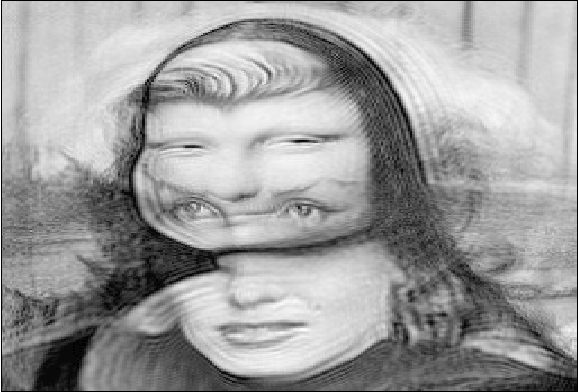
\includegraphics[width=\linewidth]{img/main.png}

\vfill
\begin{minipage}[l]{0.4\textwidth}
\large
\emph{Auteur :}\\
\@author\\
\end{minipage}
\hfill
\begin{minipage}[r]{0.4\textwidth}
\large
\flushright
\emph{A l'attention de :} \\
Carole \textsc{Le Guyader}\\ % Supervisor's Name
Vincent \textsc{Duval}\\
\end{minipage}
\newpage
}
\makeatother
%%%


%\begin{center}
%\vspace{2ex}
%{\huge \textsc{\@title}}
%\vspace{1ex}
%\\
%\linia\\
%\@author \hfill \@date
%\vspace{4ex}
%\end{center}

%\begin{tcolorbox}[enhanced,attach boxed title to top center={yshift=-3mm,yshifttext=-1mm},
 % colback=blue!5!white,colframe=blue!75!black,colbacktitle=red!80!black,
  %title=My title,fonttitle=\bfseries,
  %boxed title style={size=small,colframe=red!50!black} ]
  %This box uses a \textit{boxed title}. The box of the title can
  %be formatted independently from the main box.
%\end{tcolorbox}









\setlength{\parindent}{0pt}
\newcommand\titre{OT}
\newcommand\auteur{Timothée \textsc{Schmoderer}}
\newcommand\dateDoc{2017/2018}
\newcommand\chapitre{Chapitre 2}
\newcommand\cours{PFE}
\usepackage{enumitem}
\everymath{\displaystyle}

\title{\titre }
\author{\auteur}
\date{\dateDoc}

\usepackage{fancyhdr,lastpage}
\pagestyle{fancy}

\lhead{\cours}
\chead{}
\rhead{\currentname}
\lfoot{\titre}
\cfoot{}
\rfoot{Page \thepage\ /\ \pageref*{LastPage}}  


\lstset{
language=Matlab,
}

\hypersetup {
 pdftitle={\titre},    % title
    pdfauthor={\auteur},     % author
    pdfsubject={\cours},   % subject of the document
    pdfkeywords={}, % list of keywords
}


\renewcommand{\lstlistingname}{Code}% Listing -> Code
\renewcommand{\lstlistlistingname}{Liste des \lstlistingname s}% List of Listings -> List of codes



\begin{document}
\thispagestyle{empty}
\maketitle
\tableofcontents
\newpage

\section{Pbm de transport optimal}
Soient deux densités $f_0$ et $f_1$ de même masse, suffisamment régulière, sur un domaine $[0,1]^d$.\\
Un transport de $f_0$ sur $f_1$ est une application $T$ telle que :
$$
f_0(x)=f_1(T(x))|det(\partial T(x))|
$$
Le transport optimal est celui qui minimise le coût $\int c(x,T(x)dx$ parmi tous les transports de $f_0$ sur $f_1$. Dans notre problème : $C(x,y) =\|x-y\|^2$. 

\section{Formulation de Benamou et Brenier}
On montre que la géodésique entre $f_0$ et $f_1$ est : 
$$
f(x,t)=f_0((1-t)Id+tT(x))|det((1-t)Id+t\partial T(x))|
$$
et que ce chemin minimise le problème suivant : 
$$
\min_{(f,v)\in C_v} \int_{[0,1]^d}\int_0^1 f(x,t)\|v(x,t)\|^2dtdx
$$

Où : $C_v= \{(f,v)|\partial_t f+div_x(v)=0;v(0,.)=0,v(1,.)=0,f(.,0)=f_0,f(.,1)=f_1\}$

On pose $m = fv$ pour obtenir le problème de minimisation 
$$
\min_{(f,m)\in C}J(m,f)=\int_{[0,1]^d}\int_0^1 \theta (m,f)dtdx
$$
avec $\theta (m,f) = \frac{\|m\|^2}{f} si f>0 \quad 0 si (m,f)=(0,0)\quad \infty sinon$

Rq : on a ramené le pbm de transport optimal à celui de trouver la géodésique entre les deux densités. 
\section{Méthodes numériques}
On présente le cas 1D qui nous a accaparé. \\
Carré espace temps : $[0,1]^2$ que l'on discrétise : 
$$
G_c = \{(x_i=\frac{i}{N},t_j=\frac{j}{P})|0\leq i\leq N,\ 0\leq j\leq P\}
$$
On notre $E_c =(\RR^2)^{G_c}$ l'espace des variables centrées et $ V=(m_{ij},f_{ij}) \quad 0\leq i\leq N,\ 0\leq j\leq P$ les variables discrétisées. \\

Dans le but de capturer l'équation de continuité, on introduit une grille décentrée : 
$$
G_s^x = \{(x_i=\frac{i+1/2}{N},t_j=\frac{j}{P})|-1\leq i\leq N,\ 0\leq j\leq P\}
$$
et 
$$
G_s^t = \{(x_i=\frac{i}{N},t_j=\frac{j+1/2}{P})|0\leq i\leq N,\ -1\leq j\leq P\}
$$

On note $E_s=\RR^{G_s^x}\times\RR^{G_s^t}$ l'espace des variables décentrées, et $U=(\bar{m_{ij}}\quad 1\leq i\leq N,\ 0\leq j\leq P,\bar{f_{ij}},\quad 0\leq i\leq N,\ -1\leq j\leq P$


\section{Opérateurs}
On introduit plusieurs opérateurs pour lier les variables décentrées et les variables centrées.
\subsection{Interpolation}
$$
I:E_s \rightarrow E_c
$$
tq 
$$
m_{ij} = = (\bar{m}_{i+1/2,j}+\bar{m}_{i-1/2,j})/2.
$$
et
$$
f_{ij} = = (\bar{f}_{i,j+1/2}+\bar{f}_{i,j-1/2})/2.
$$
Cet opérateur s'interprète matriciellement : 
$$
m = \bar{m}I_m
$$
et 
$$
f = I_f\bar{f}
$$

\subsection{Divergence}
l'opérateur qui approxime la divergence
$$
div : E_s\rightarrow \RR^{G_c}
$$
et 
$$
div(\bar{m},\bar{f})_{ij} = (\bar{m}_{i+1/2,j}-\bar{m}_{i-1/2,j}) + (\bar{f}_{i,j+1/2}-\bar{f}_{i,j-1/2})
$$

\subsection{Frontières}
Un opérateur pour extraire les frontières : 

$$
b(\bar{m},\bar{f}) = ((\bar{m}_{-1/2,j},\bar{m}_{N+1/2,j});(\bar{f}_{i,-1/2},\bar{f}_{i,P+1/2}))
$$
et on impose les conditions aux frontières suivantes : 
$$
b(\bar{m},\bar{f}) = b_0=(0,0,f_0,f_1);
$$

\subsection{Problème discrétisé}

On a le problème suivant 

$$
\min_{U=(\bar{m},\bar{f})\in E_s} \theta(I(\bar{m},\bar{f})) + \iota_C(U)
$$
avec l'ensemble des contraintes :
$$
C=\{(\bar{m},\bar{f})\in E_s|\ div(\bar{m},\bar{f}) = 0\ b(\bar{m},\bar{f}) = b_0 \}
$$

\section{Résolution par algorithme de séparation de proximité}
Ces algorithmes sont des généralisation des algos de gradient conjugués. \\

\textbf{Remarque : } On a $J(m,f)=\int_{[0,1]^d}\int_0^1 \frac{\|m\|^2}{f} dtdx$ donc si $f\rightarrow\infty$ on a $J\rightarrow 0$ donc ce n'est pas coercif ce qui rend l'existence de minimiseurs non triviale. Et si $f\rightarrow 0$, on a $j\rightarrow \infty$ donc les méthodes de gradient conjugués ne peuvent pas s'appliquer, le gradient n'est pas lipschitz. \\

On veut résoudre le pbm suivant : 
$$
\min_{z=(U,V)\in E_s\times E_c} G_1(z)+G_2(z)
$$
où, $G_1(z) = J(U)+\iota_C(U)$ et $G_2(z)=\iota_{C_s}(z)$ et $C_s=\{z=(U,V)\in E_s\times E_c\ | \ V=I(U) \}$


\remarque{$G_1$ est la fonctionnelle originelle et $G_2$ vient de notre introduction des variables décalées. }\\

On va alors calculer les opérateurs de proximités de $G_1$ et $G_2$.On dit que $G_1$ est \textbf{simple} dans la mesure ou : 

$$
Prox_{\gamma G_1} (U,V) = (Prox_{\gamma C} (U),Prox_{\gamma J} (V))
$$

\subsection{Opérateur de proximité de $G_2$}

$$
Prox_{\gamma C_s} (U,V) = arg\min_{z'\in C_s} \frac{1}{2}\|z-z'\|^2= Proj_{C_s}(U,V)
$$
Suivant l'article de Papadakis, Peyré et Oudet on a :

$$
Prox_{\gamma C_s} (U,V)  = (\tilde{U},I(\tilde{U}))
$$
et 

$$
\tilde{U} = (Id +I^{\star}I)^{-1}(U+I^{\star}(V))
$$
Ou $I^{\star}$ est l'adjointe de $I$. ce qui nous donne en terme de matrice : 
$$
\tilde{\bar{m}} = (\bar{m}+mI_m^{\star})(Id +I_mI_m^{\star})^{-1}
$$
et 
$$
\tilde{\bar{f}} = (Id +I_f^{\star}I_f)^{-1}(\bar{f}+I_f^{\star}f)
$$
enfin : $\tilde{m}=\tilde{\bar{m}}I_m$ et $\tilde{f}=I_f\tilde{\bar{f}}$

Comme l'opérateur d'interpolation s'interprète matriciellement, son adjoint est donné par la transposée. 

\subsection{Opérateur de proximité de $J$}

$Prox_{\gamma J}(V)=(Prox_{\gamma J}(V_k))_{k\in G_c}$ et 

$$
Prox_{\gamma J}(m_k,f_k) = (\frac{f^{\star}_km_k}{f^{\star}_k+2\gamma},f^{\star}_k)\ si\ f^{\star}>0 \qquad (0,0)\ sinon
$$ 
et $f^{\star}_k$ est la plus grande racine réelle du polynôme de degré 3 donné par : 
$$
P(x) = (X-f_k)(X+2\gamma)^2-\gamma \|m_k\|^2
$$
La racine est calculée rapidement avec l’algorithme de Newton. 

\subsection{Opérateur de proximité de $\iota_C$}

$$
Prox_{\gamma C} = Proj_C
$$
on réécrit l'ensemble des contraintes sous la forme : 

$$
C=\{U\in E_s\ | \ AU=y\} \qquad A=(div,b)^T \qquad y = (0,b0)^T
$$

et on obtient $Proj_C(U)=(Id +A^{\star}\Delta^{-1}A)U + A^{\star} \Delta^{-1}y$ avec $\Delta^{-1}=(A^{\star}A)^{-1}$ et son problème requiert la résolution d'un problème de poisson. 

\section{Algorithme de Douglas Rachford}
On procède à l'itération suivante : $(z^l,w^l)\in (E_s\times E_c)\times (E_s\times E_c)$ avec un $w^0$ donné : 
$$
z^{l+1}=Prox_{\gamma G_2} (w^l)
$$
et 
$$
w^{l+1}=(1-\frac{\alpha}{2})w^l + \frac{\alpha}{2}RProx_{\gamma G_2}\circ RProx_{\gamma G_1} (w^l)
$$

Où on a posé : $RProx_{\gamma G} = 2Prox_{\gamma G}-Id$.\\
On montre alors que pour $\alpha\in ]0,2[$ et $\gamma>0$ la méthode converge $z^l\rightarrow z^{\star}$ ce qui permet de retrouver la géodésique, car : 
$$
z^l=(U^l,V^l)\rightarrow (U^{\star},V^{\star}) \qquad V^{\star}=(m^{\star},f^{\star})
$$

\newpage
\addcontentsline{toc}{section}{\listfigurename}
\listoffigures
\addcontentsline{toc}{section}{\lstlistlistingname}
\lstlistoflistings


\end{document}
